% Options for packages loaded elsewhere
\PassOptionsToPackage{unicode}{hyperref}
\PassOptionsToPackage{hyphens}{url}
%
\documentclass[
  english,
  jou]{apa6}
\usepackage{amsmath,amssymb}
\usepackage{lmodern}
\usepackage{iftex}
\ifPDFTeX
  \usepackage[T1]{fontenc}
  \usepackage[utf8]{inputenc}
  \usepackage{textcomp} % provide euro and other symbols
\else % if luatex or xetex
  \usepackage{unicode-math}
  \defaultfontfeatures{Scale=MatchLowercase}
  \defaultfontfeatures[\rmfamily]{Ligatures=TeX,Scale=1}
\fi
% Use upquote if available, for straight quotes in verbatim environments
\IfFileExists{upquote.sty}{\usepackage{upquote}}{}
\IfFileExists{microtype.sty}{% use microtype if available
  \usepackage[]{microtype}
  \UseMicrotypeSet[protrusion]{basicmath} % disable protrusion for tt fonts
}{}
\makeatletter
\@ifundefined{KOMAClassName}{% if non-KOMA class
  \IfFileExists{parskip.sty}{%
    \usepackage{parskip}
  }{% else
    \setlength{\parindent}{0pt}
    \setlength{\parskip}{6pt plus 2pt minus 1pt}}
}{% if KOMA class
  \KOMAoptions{parskip=half}}
\makeatother
\usepackage{xcolor}
\IfFileExists{xurl.sty}{\usepackage{xurl}}{} % add URL line breaks if available
\IfFileExists{bookmark.sty}{\usepackage{bookmark}}{\usepackage{hyperref}}
\hypersetup{
  pdftitle={An open-source implementation of the computer adaptive philadelphia naming test},
  pdfauthor={Alexander M Swiderski1, 2 \& Robert Cavanaugh1,2},
  pdflang={en-EN},
  pdfkeywords={aphasia, computer, adaptive, naming, test},
  hidelinks,
  pdfcreator={LaTeX via pandoc}}
\urlstyle{same} % disable monospaced font for URLs
\usepackage{graphicx}
\makeatletter
\def\maxwidth{\ifdim\Gin@nat@width>\linewidth\linewidth\else\Gin@nat@width\fi}
\def\maxheight{\ifdim\Gin@nat@height>\textheight\textheight\else\Gin@nat@height\fi}
\makeatother
% Scale images if necessary, so that they will not overflow the page
% margins by default, and it is still possible to overwrite the defaults
% using explicit options in \includegraphics[width, height, ...]{}
\setkeys{Gin}{width=\maxwidth,height=\maxheight,keepaspectratio}
% Set default figure placement to htbp
\makeatletter
\def\fps@figure{htbp}
\makeatother
\setlength{\emergencystretch}{3em} % prevent overfull lines
\providecommand{\tightlist}{%
  \setlength{\itemsep}{0pt}\setlength{\parskip}{0pt}}
\setcounter{secnumdepth}{-\maxdimen} % remove section numbering
% Make \paragraph and \subparagraph free-standing
\ifx\paragraph\undefined\else
  \let\oldparagraph\paragraph
  \renewcommand{\paragraph}[1]{\oldparagraph{#1}\mbox{}}
\fi
\ifx\subparagraph\undefined\else
  \let\oldsubparagraph\subparagraph
  \renewcommand{\subparagraph}[1]{\oldsubparagraph{#1}\mbox{}}
\fi
% Manuscript styling
\usepackage{upgreek}
\captionsetup{font=singlespacing,justification=justified}

% Table formatting
\usepackage{longtable}
\usepackage{lscape}
% \usepackage[counterclockwise]{rotating}   % Landscape page setup for large tables
\usepackage{multirow}		% Table styling
\usepackage{tabularx}		% Control Column width
\usepackage[flushleft]{threeparttable}	% Allows for three part tables with a specified notes section
\usepackage{threeparttablex}            % Lets threeparttable work with longtable

% Create new environments so endfloat can handle them
% \newenvironment{ltable}
%   {\begin{landscape}\begin{center}\begin{threeparttable}}
%   {\end{threeparttable}\end{center}\end{landscape}}
\newenvironment{lltable}{\begin{landscape}\begin{center}\begin{ThreePartTable}}{\end{ThreePartTable}\end{center}\end{landscape}}

% Enables adjusting longtable caption width to table width
% Solution found at http://golatex.de/longtable-mit-caption-so-breit-wie-die-tabelle-t15767.html
\makeatletter
\newcommand\LastLTentrywidth{1em}
\newlength\longtablewidth
\setlength{\longtablewidth}{1in}
\newcommand{\getlongtablewidth}{\begingroup \ifcsname LT@\roman{LT@tables}\endcsname \global\longtablewidth=0pt \renewcommand{\LT@entry}[2]{\global\advance\longtablewidth by ##2\relax\gdef\LastLTentrywidth{##2}}\@nameuse{LT@\roman{LT@tables}} \fi \endgroup}

% \setlength{\parindent}{0.5in}
% \setlength{\parskip}{0pt plus 0pt minus 0pt}

% \usepackage{etoolbox}
\makeatletter
\patchcmd{\HyOrg@maketitle}
  {\section{\normalfont\normalsize\abstractname}}
  {\section*{\normalfont\normalsize\abstractname}}
  {}{\typeout{Failed to patch abstract.}}
\patchcmd{\HyOrg@maketitle}
  {\section{\protect\normalfont{\@title}}}
  {\section*{\protect\normalfont{\@title}}}
  {}{\typeout{Failed to patch title.}}
\makeatother
\shorttitle{computer adaptive philadelphia naming test}
\keywords{aphasia, computer, adaptive, naming, test\newline\indent Word count: 720}
\usepackage{dblfloatfix}


\usepackage{csquotes}
\ifXeTeX
  % Load polyglossia as late as possible: uses bidi with RTL langages (e.g. Hebrew, Arabic)
  \usepackage{polyglossia}
  \setmainlanguage[]{english}
\else
  \usepackage[main=english]{babel}
% get rid of language-specific shorthands (see #6817):
\let\LanguageShortHands\languageshorthands
\def\languageshorthands#1{}
\fi
\ifLuaTeX
  \usepackage{selnolig}  % disable illegal ligatures
\fi

\title{An open-source implementation of the computer adaptive philadelphia naming test}
\author{Alexander M Swiderski\textsuperscript{1, 2} \& Robert Cavanaugh\textsuperscript{1,2}}
\date{}


\authornote{

Add complete departmental affiliations for each author here. Each new line herein must be indented, like this line.

Enter author note here.

Correspondence concerning this article should be addressed to Alexander M Swiderski, Postal address. E-mail: \href{mailto:my@email.com}{\nolinkurl{my@email.com}}

}

\affiliation{\vspace{0.5cm}\textsuperscript{1} University of Pittsburgh\\\textsuperscript{2} VA Pittsburgh Healthcare System}

\abstract{
The Phialdelphia Naming Test (Roach et al., YEAR) is a good naming test. However it is very long because classical test theory. Previous work created a computer adaptive philadelphia naming test using item response theory. IRT is super cool. But the previous software was in Java and was not ideal for sharing. Also it needed to be updated. Therefore, we made a version using free, open-source software Shiny and have made it available. Woot woot. We did some testing at it works great. It's easy to use. you can use it online or locally. The code is available. We discuss how you might use it. Go us.
}



\begin{document}
\maketitle

\hypertarget{introduction}{%
\section{Introduction}\label{introduction}}

The Philadelphia Naming Test (PNT; Roach et al., 1996) is a 175 item picture naming test utilized to assess anomia in people with aphasia. It is made up of diverse stimuli varying in length, age of acquisition, and lexical frequency (Francis \& Kucera, 1982), it has a well-defined scoring system for classifying anomic errors (Dell et al., 1997), and its total score correlates highly with aphasia severity (Walker \& Schwartz, 2012). The PNT was developed in a classical test theory framework (Traub, 1997). There are two primary outcomes measures that can be utilized to score the original PNT. First, an overall accuracy score. Second, the total number of response types observed. The former scoring type provides an overall estimate of anomia severity, and the total number of response types can be utilized to make inference on the underlying lexical-semantic and lexical-phonological abilities.

Despite the widespread use of confrontation picture naming tests, their utility for quantifying anomia is limited due to their construction with classical test theory. For example, the standard error is considered constant across all items regardless of the items difficulty or the participants naming ability. This assumption ignores that measurement error varies as a function of item difficulty and naming ability. To illustrate this point, consider the following example. If a test were administered to a group of people with very mild anomia that only included very easy items they would all likely score perfectly. Therefore, rank ordering these participants based on their naming ability would not be possible. However, if a test of more difficult items were delivered to the same group of people with aphasia, it is less likely they would all perform perfectly and rank ordering the individuals would be possible.

Item Response Theory (IRT; De Ayala, 2009; Lord, 1980) is a modern psychometric theory that formalizes the probability of a correct response given an items difficulty and the participants ability. difficulty can be conceptualized as the ease or challenge of producing a correct response and ability is operationalized as the degree to which an individual possesses a certain skill. As it pertains to the assessment results from the PNT accessed through this shiny application (Chang et al., 2021) difficulty and ability reflect the degree of naming difficulty and degree of degree of naming impairment, respectively. In IRT applications the range of both difficulty and ability ranges from -4 to 4.

As it pertains to this application, our research group first estimated the 1-Parameter logistic (1-PL) model (a utility of IRT) with archival data (Mirman et al., 2010) from 251 participants with aphasia (Fergadiotis Gerasimos et al., 2015). The 1-PL model is expressed as follows:

{[}formula 1{]}

Where the probability of (P) of a correct response by examine j with a naming ability {[}THETA{]} is equal to a log transformation of the participants naming ability minus the item's difficulty {[}BETA{]}. Note that {[}ALPHA{]} is the item discrimination parameter, which is assumed to be equal for all items under the assumptions of the 1-pl model.

Item characteristic curves can then be estimated for each item for all possible ability levels. Item characteristic curves are sigmoidal in shape and are presented for the following items in Figure 1: Ambulance, ball, and microscope. Note that zero is considered the average naming ability estimate. As can be extracted from the figure, a participant with a naming ability has a probability of responding correctly to ambulance, ball, and microscope of roughly 0.33, 0.80, and 0.15 respectively For an interactive application that can be utilized to plot item characteristic curves for any item on the PNT see \url{https://aswiderski.shinyapps.io/IRTapp/}.

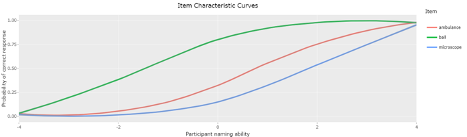
\includegraphics{fig1.png}

The amount of information that each item carries about a given naming ability is formalized by the item information function and information is maximized when the item's difficulty matches the participants ability. Information is formalized as:

{[}formula 2{]}

where the information for item i is the product of the probability of a correct response for an individual with an ability of {[}THETA{]} multiplied by the probability of an incorrect response for item i from an individual with an ability of {[}THETA{]}. In the IRT framework, the standard error is the inverse of the information function:

{[}formula 3{]}

Therefore, the more information an item provides the less measurement error is present.

Next sections:

\begin{itemize}
\tightlist
\item
  Computer adaptive testing
\item
  PNT-CAT30
\item
  PNT-CATVL
\item
  Should we include a FAQ page?
\item
  Screenshots?
\end{itemize}

\hypertarget{references}{%
\section{References}\label{references}}


\end{document}
